\chapter{Растяжение воображения}


\setlength{\epigraphwidth}{.80\textwidth}
\epigraph{Не стоит доверять глазам, когда разыгралось воображение.
}{--- Марк Твен (1835---1910), Янки при дворе короля Артура}

Следующие головоломки потребуют от вас разработки \emph{плана},
и иногда придётся напрячь воображение!

\subsection*{Любовь в Клептопии}\rindex{Любовь в Клептопии}\label{Любовь в Клептопии}

Ян влюбился в Марию (по интернету), и он хочет послать ей кольцо.
Однако они живут в Клептопии, стране где всё, что отправляется по почте, будет неминуемо украдено, если только не отправлено в ящике запертом на навесной замок.
У Яна и Марии много замков, но ни у кого из них нет ключа к замку другого.
Как им переслать кольцо?

\subsection*{Черви и вода}\rindex{Черви и вода}\label{Черви и вода}

Лори надоело, что черви забираются к ней на кровать.
Она поставила ножки кровати в вёдра с водой;
поскольку черви не умеют плавать, они не могут добраться до кровати по полу.
Однако теперь они ползут вверх по стенам и по потолку, и падают на кровать сверху.
Фу!

Как защититься от червей?

\parit{Примечания.}
Можно попробовать соорудить навесную конструкцию над кроватью.
Для того чтобы предотвратить падение червей на навес,
их дальнейшее проползание по навесу
и падение на кровать, возможно, стоит сделать жёлоб вокруг навеса и наполнить его водой.
Но ведь тогда черви смогут упасть на край желоба.
Хм...

\subsection*{Проверка страусиных яиц}\rindex{Проверка страусиных яиц}

В преддверии рекламной кампании страусиной ферме нужно проверить яйца своих страусов на прочность.
В мировой практике прочность определяют по самому высокому этажу Эмпайр-стейт-билдинга, с которого можно сбросить яйцо так, чтоб оно не разбилось.

Официальный инспектор фирмы, Оскар, понимает, что если он возьмёт с собой в Нью-Йорк одно яйцо,
то для определения прочности придётся (возможно) бросить его с \emph{каждого} из 102 %101???
этажей, начиная с первого.
А что если он возьмёт \emph{два} яйца?
Сколько бросков ему потребуется в худшем случае?

\begin{addedbytheeditors}
\textbf{Редакторам:}
Тут возникает проблема с американской и русской нумерацией этажей + похоже, что Уинклер считает, что нет смысла бросать яйцо с нулевого этажа.
\end{addedbytheeditors}


\subsection*{Опасная картина}\rindex{Опасная картина}

Требуется повесить картину за шнур прикреплённый к раме.
Если это сделать как обычно, перекинув шнур через два гвоздя как показано на рисунке, и один из гвоздей выпадет, то картина останется висеть на другом гвозде (хотя и накренится).

Можно ли повесить картину так, чтобы она упала, если выпадет \emph{любой} из двух гвоздей?

\begin{figure}[h!]
\centering
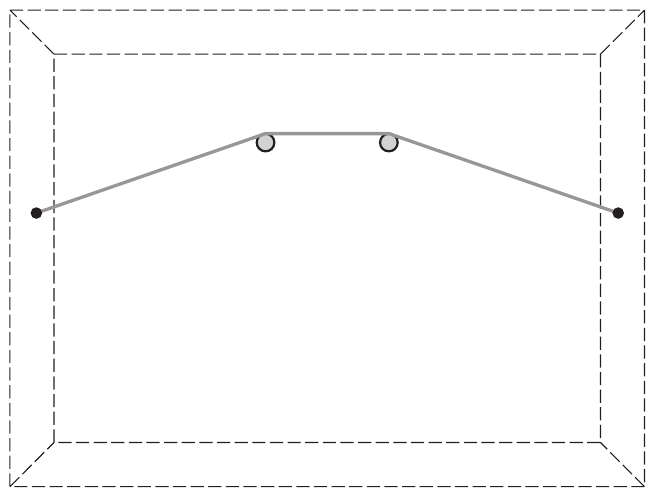
\includegraphics[scale=0.5]{pics/kartina1}
\caption{Эта картина останется висеть если выпадет один гвоздь.}
\label{pic:kartina1}
\end{figure}

\subsection*{Замок с дефектом}\rindex{Замок с дефектом}\label{Замок с дефектом}

Кодовый замок имеет три диска, с положениями пронумерованными от 1 до 8.
У замка есть дефект, чтобы его открыть, достаточно правильно выставить два числа из трёх.
Какое минимальное число (трёхзначных) комбинаций достаточно проверить, чтобы точно открыть замок?

\parit{Примечания.}
Есть много способов проделать это $64$-мя тестовыми комбинациями, например, можно перебрать все возможные варианты первых двух дисков или проверить все комбинации, сумма значений которых кратна 8.
Однако каждая тройная комбинация охватывает $22$ возможных случая, а всего комбинаций $8^3 = 512$. 
Поэтому в принципе хватить $\lceil 512/22 \rceil = 24$ тестовых комбинаций.
То есть истина где-то между $24$ и $64$; вопрос где?

\subsection*{Альтернативные кубики}\rindex{Альтернативные кубики}

 
Можно ли изготовить такую пару игральных кубиков, чтобы их суммы вели себя так же, как у пары обычных кубиков?
То есть должно быть два способа выбросить 3, шесть способов выбросить 7, один способ выбросить 12 и так далее.
У кубиков должно быть по шесть граней, и на каждой грани должно быть указано положительное целое число.

\subsection*{Совпадение монет}\rindex{Совпадение монет}

Сонни и Шер играют в следующую игру.
В каждом раунде бросается честная монета.
Перед броском Сонни и Шер одновременно объявляют свои предположения о результате броска.
Они выигрывают раунд, если оба угадали правильно.
Требуется максимизировать долю выигранных раундов, предполагая, что игра идёт долго.

Пока что ответ очевиден --- 50\%: Сонни и Шер договариваются о последовательности предположений (например, всегда говорить «орёл»).
Очевидно, что лучшего им не добиться.

Однако перед началом игры игрокам сообщается, что Шер получит результаты всех бросков монеты заранее, прямо перед первым броском!
У неё есть возможность обсудить стратегию с Сонни заранее, но как только она получит данные о бросках, возможности передавать информацию больше не будет.
Можно ли добиться 70\%-й доли выигрышей?

\subsection*{Имена в ящиках}\rindex{Имена в ящиках}\label{Имена в ящиках}

Имена 100 заключённых помещают в 100 деревянных ящиков, по одному в каждом;
ящики расставляются в ряд на столе в комнате.
Заключённых приводят в комнату поочерёдно;
каждому позволяется заглянуть не более, чем в 50 ящиков,
затем он должен покинуть комнату, оставив её в точно том же состоянии как и до прихода,
и дальнейшее общение невозможно.

У заключённых есть возможность спланировать свою стратегию заранее, и им это понадобится --- если хотя бы один заключённый не найдёт своё имя, то казнят всех.
Найдите стратегию, вероятность успеха которой превысит 30\%.

\parit{Примечания.} Если каждый заключённый откроет случайный набор из 50 ящиков, то вероятность выжить составлит незавидные
\[(\tfrac12)^{100}\z\sim 0{,}0000000000000000000000000000008.\]
Но они могут поступить и хуже --- если все откроют одни и те же 50 ящиков, то их шансы упадут до нуля.
Но тридцать процентов уж совсем недостижимы...
Очень хорошо --- вы правильно поняли задачу!
